%%%%%%%%%%%%%%%%%%%%%%%%%%%%%%%%%%%%%%%%%%%%%%
\logvartrue
\chapter{Bacteria-environment interaction}
%%%%%%%%%%%%%%%%%%%%%%%%%%%%%%%%%%%%%%%%%%%%%%
Microscopic bacteria are usually considered one of the most simple and primitive living species. In the popular mind, they are associated almost exclusively with infection diseases or with the bio-degradation of organic matter. But reality is different, hence, within a highly diversified and beneficial bacterial world, only a very small fraction is able to cause infections. Most of known bacterial ``species'' reciprocally support each other and are able to define and sustain a balanced environment, the so-called biosphere. This ``solidarity'' among bacterial cells is one of their  most important characteristics. Indeed, even pathogenic bacteria are able to benefit from these mutual interactions, helping themselves to be more flexible than if they lived as isolated species. For these reasons studying the relations between bacteria and their environment by identifying their community structure is becoming more and more considered as a mandatory step towards the comprehension of the biological dynamics existing on our planet.\\
These topics have been discussed in the following paper:
\vspace{-2mm}
\begin{itemize}[nosep]
\item \textbf{Bacci, G.}, Ceccherini, M.T., Bani, A., Bazzicalupo, M., Castaldini, M., Galardini, M., Giovannetti, L., Mocali, S., Pastorelli, R., Pantani, O.L., Arfaioli, P., Pietramellara, G., Viti, C., Nannipieri, P., \& Mengoni, A. Exploring the dynamics of bacterial community composition in soil: the pan-bacteriome approach.
\end{itemize}
that has been accepted for publication in \textit{Antonie van Leeuwenhoek}.

\section[Exploring the dynamics of bacterial community composition in soil: the pan-bacteriome approach]{Exploring the dynamics of bacterial community composition in soil: the pan-bacteriome approach%
\sectionmark{The pan-bacteriome approach}}
\sectionmark{The pan-bacteriome approach}
We performed a longitudinal study (repeated observations of the same sample over time) to investigate both the composition and structure of temporal changes of bacterial community composition in soil mesocosms, subjected to three different treatments (water and 5 mg kg\textsuperscript{-1}, 25 mg kg\textsuperscript{-1} of dried soil Cd\textsuperscript{2+}). By analogy with the pan genome concept, we identified a core bacteriome and an accessory bacteriome. Resident taxa were assigned to the core bacteriome, while occasional taxa were assigned to the accessory bacteriome. Core and accessory bacteriome represented roughly 35\% and 50\% of the taxa detected, respectively, and were characterized by different taxonomic signatures from phylum to genus level while the 15\% of the taxa were found to be unique to a particular sample. In particular, the core bacteriome was characterized by higher abundance of \textit{Planctomycetes}, \textit{Actinobacteria}, \textit{Verrucomicrobia} and \textit{Acidobacteria}, while the accessory bacteriome included more members of \textit{Firmicutes}, \textit{Clamydiae} and \textit{Proteobacteria}, suggesting potentially different responses to environmental changes of members from these phyla. We conclude that the pan-bacteriome model may be a useful approach to gain insight for modelling bacterial community structure and inferring different abilities of bacteria taxa.\\

\subsection{Introduction}
Understanding changes in bacterial community structure over time is still one of the major challenges in microbial ecology \cite{ge2008differences, zhou2014stochasticity, donn2014evolution}. Indeed, environmental changes often affect taxonomic composition and abundance in microbial communities \cite{allison2008resistance}, which may have a strong effect on soil health and plant productivity \cite{chaparro2012manipulating}. Several works have been performed inspecting bacterial community variation both in cross sectional (different sites at the same time) and longitudinal studies (the same site studied over time) \cite{costello2009bacterial, pini2012exploring, smith2012cervical, bartram2014exploring, logares2012biogeography, chen2013shifts, kuang2012contemporary}.\\
A pan-genome is defined as the collection of all the genes of a set of bacteria which can be divided into core genome (the group of genes shared by all the selected bacteria), accessory genome (the group of genes present in some, but not all, of the selected bacteria) and unique genome (genes belonging to only one particular strain) \cite{tettelin2008comparative}. In analogy with this concept we can define a pan-bacteriome as the collection of all bacterial taxa present in a set of environmental samples. As recently reported \cite{hardoim2014temporal}, the pan-bacteriome can be divided into the core bacteriome (the pool of taxa shared by all the samples), the accessory bacteriome (the group of taxa found in some, but not all the samples) and the unique bacteriome (taxa detected only in a particular sample).\\
Several recent works \cite{bartram2014exploring, logares2012biogeography, bowen2012salt, aravindraja2013ultradeep, dohrmann2012importance, gibbons2013evidence, kim2013general, oh2013altered, portillo2013cell, sanchez2013assessing, szekely2014importance, wegner2013disturbance}, mainly performed with next generation sequencing technologies, have demonstrated that most bacterial communities are composed of a few abundant taxa and a plethora of rare ones \cite{pedros2012rare}. Such different fractions may have in theory different taxonomic signatures (at the various taxonomic levels), in relation to the physiological features of the groups of taxa present. For these reasons, we define the ``pan-bacteriome'' concept, as the whole set of taxa present in a bacterial community analyzed through multiple samplings through time. The pan-bacteriome will then include both a core and an accessory fraction, which describe the taxa shared by all samples and the taxa present only in some samples, respectively. In addition, the so called ``rare biosphere'', composed by taxa occurring only in a fraction of the community samples, and interpreted as the accessory fraction of the bacterial community, seems more readily respond to environmental changes \cite{dohrmann2012importance, kim2013general, szekely2014importance, campbell2011activity, gobet2011diversity}.\\
Contaminated soils have been often used as models for inspecting bacterial evolution over time \cite{mengoni2010plants, porter2013trade}, since different bacterial taxa show different responses to contamination. The most oxidized state (and most frequent) of cadmium (Cd\textsuperscript{2+}) is known to be toxic for soil microbial biomass and activity \cite{renella2002cadmium, renella2005microbial} and several studies have shown that Cd\textsuperscript{2+} concentrations affect soil microbial diversity under short-term cadmium stress \cite{gomes2010effects, lorenz2006response, chien2008microbial, duan2008effect, lazzaro2008identification, sheoran2008remediation, zhang2009responses, fritze2000effect}. The aim of this work was to apply the pan-bacteriome model, as sum of a core and an accessory assemblage of bacteria taxa present in bacterial communities, to evaluate the dynamics of bacterial community composition in three soil mesocosms, exposed to slightly different environmental conditions (concentrations of 0, 5 mg kg\textsuperscript{-1} and 25 mg kg\textsuperscript{-1} of dried soil Cd\textsuperscript{2+}) through time. A metabarcoding approach was applied on 16S rRNA gene based on Illumina sequencing technology.\\

\subsection{Materials and Methods}

\subsubsection{Experimental setup}
The top layer (0-15 cm) of a soil located near Romola (Florence, Italy 43.696240 N, 11.153894 E) was sampled (about 20 kg), air-dried overnight at room temperature and sieved at 2 mm. The sieved air-dried soil mass was repeatedly split to ensure the representativeness of the initial material, which was finally divided into masses of about 1 Kg each. One mass was analyzed for relative humidity (RH 7.30\%), particle size (sand 81.9\%; silt 6.7\%; clay 11.4\%), water holding capacity (WHC 14.85 g 100 g\textsuperscript{-1} of dried soil), pH (5.4), total organic C (0.7\%), and organic N (0.07\%) after the air-drying process and just before the constitution of the mesocosms.\\
Three of the remaining masses were used to constitute the mesocosms. Each mesocosm was formed by a flat-bottomed plexiglas cylinder (10 cm height, 15 cm of diameter) previously disinfected with 70\% ethanol, which contained the soil mass. Its base was perforated to permit aeration and water flow. The cylinder was supported by a similar one not perforated, intended to collect any possible leak of soil or solution. The upper part of the mesocosm was weighted, to keep track of the water losses which were reconstituted weekly throughout the experiment. Then an excess 350 ml of sterile distilled water was thoroughly and slowly dripped on the dried soil: the mesocosms were then brought to a thermostatic clean room at 22 {\textdegree}C into which they were maintained and their position rotated every third day for two months. When the mesocosms reached about the 25\% of the WHC, they were randomly assigned to one of the following treatment: A) sterile distilled water, B) 3CdSO\textsubscript{4}{\textperiodcentered}8H\textsubscript{2}O (Sigma-Aldrich) sterile solution as to reach a final concentration of 5 mg kg\textsuperscript{-1} of dried soil, C) 3CdSO\textsubscript{4}{\textperiodcentered}8H\textsubscript{2}O sterile solution as to reach a final concentration of 25 mg kg\textsuperscript{-1} of dried soil (Figure SM1). The volume and the concentration of Cd solutions were adjusted to reach both the 50\% of the soil WHC and the Cd concentration in mg kg\textsuperscript{-1} of dried soil. The mesocosms were sampled at 0, 1, 4, 8, 36 and 60 days (t0, t1, t4, t8, t36, t60) after the initial Cd solution spiking. The first sampling time (t0) took place as soon as the soil was visibly saturated with the Cd solution. On each date, a brass pipe was used to withdraw three replicates. DNA extraction was performed on each of the three soil cores (1.2 cm diameter, 6 cm deep). The location of the cores on the mesocosm surface was selected by randomly generating 1000 groups of 6 {\texttimes} 3 polar coordinates (i.e. an angle and a distance for each date and replica): if the area of the cores in two or more locations/dates overlapped or were tangent, the next group (among the 1000 generated) with more distant locations was selected. An R script was used to generate and print 1000 cardboard notched disks which were used to unambiguously locate the position of the cores, as previously described \cite{ceccherini2007effect}. A total of 54 samples (3 mesocosms, 6 sampling dates, 3 soil cores for DNA extraction (replicates) were collected (Figure SM1). All steps were performed under sterile  conditions.\\

\subsubsection{DNA extraction and 16S rRNA metabarcoding}
Each soil core was well mixed before DNA extraction. DNA was extracted from 0.5g of the cores using the bead-beating method as previously described \cite{ascher2009sequential}. The extracted DNA was checked by electrophoresis on 1\% (w/vol) agarose gel and quantified by Picodrop spectrophotometer (Picodrop Limited, UK).\\
For metabarcoding, each extracted DNA sample was amplified using primers targeting the variable V6 region of 16S rDNA (V6-967F 5'-CAA\-CGC\-GAA\-GAA\-CCT\-TAC\-C-3' and V6-1046R 5'-CGA\-CAG\-CCA\-TGC\-ANC\-ACC\-T-3' \cite{huse2008exploring}. PCR conditions were those previously described by Sogin and co-workers \cite{sogin2006microbial}. Ten independent PCR reactions for each of the 54 samples were done. Products were resolved by agarose gel (1.5\% w/vol) electrophoresis and bands were purified with MinElute Gel Extraction Kit (Qiagen, Inc.). Quality and quantity of products were assessed spectrophotometrically (Biophotometer, Eppendorf). The amplicons from each sample were pooled together and a total of 54 samples were sequenced. Massive parallel sequencing was performed by Illumina-Solexa technology \cite{bartram2011generation,gloor2010microbiome} with the pair-end protocol on an Illumina HiSeq2000 machine by Beijing Genome Institute sequencing service \href{www.genomics.cn}{www.\-gen\-omi\-cs.cn}. Sequences are deposited in SRA database under the BioProject accession number SRP038532.\\

\subsubsection{Bioinformatic processing of 16S rRNA metabarcoding data: data pretreatment}
Sequences were analyzed in order to identify and remove low quality regions. Since raw sequences had a length of 100 bp, the quality control step had to be very conservative, to prevent the removal of taxonomically significant data. As a consequence, a dynamic trimming algorithm was used \cite{bacci2014streamingtrim} setting the cutoff parameter as the mean quality of the whole files minus the standard deviation value (in this case an average quality cutoff of 33 Phred was used for all files \cite{ewing1998base, ewing1998base}). Collected sequences were subjected to a further quality control step and assembled using PANDAseq \cite{masella2012pandaseq}. Finally, a set of 18,778,601 sequences (mean length 112 bp and overlapping for more than 70 bp, data not shown) was achieved and used for successive analyses. In order to assign each read to specific taxa we used the RDP multiclassifier trained on the default RDP dataset (16S training set 9). An assignment cutoff of 0.5 was used as reported in the RDP Classifier pipeline for sequences shorter than 250 bp \cite{wang2007naive}.\\

\subsubsection{Data treatment and statistical analysis}
RDP assignments at all taxonomic levels (from phylum to genus) were collected. The average number of assignments in all samples was evaluated. RDP assignments were collected for each sample to generate a community data matrix (\textit{X}) at genus level (rows = samples; columns = detected genera) (Table SM1). \textit{X} was used as the input/source for all statistical analyses. In order to detect genera belonging to the core and to the accessory bacteriome, \textit{X} was transformed into a Boolean (presence/absence) matrix (\textit{X}\textit{\textsubscript{p/a}}). Abundance values greater than or equal to 1 were rounded to 1 while abundance values equal to 0 were left unchanged. Each genus was assigned to one of the core or to the accessory bacteriome fractions using these criteria: if a genus was detected in all samples (its abundance value was greater than 0 in the 54 samples) it was assigned to the core bacteriome; otherwise it was assigned to the accessory bacteriome. In addition, if a genus was detected only in a single sample, it was considered as ``unique assignment''.\\
To assess taxa richness, a rarefaction analysis was performed using the R package Vegan \cite{oksanen2007vegan, dixon2003vegan}, based on the genus assignments in \textit{X}. The variation in the composition of bacterial communities with respect to conditions and time was analyzed by canonical correlation analysis (CCA) using the R package Vegan on \textit{X}. The different conditions and the sampling times have been fitted onto previously developed ordination analyses using the \textit{envfit} function of the R package Vegan with 10'000 permutations.\\

\subsection{Results}

\subsubsection{Description of sequence data and coverage}
A total of 18,778,601 reads were processed for the 54 sequence files representing each of the samples (Figure SM1). The reads in the sequence files ranged from a minimum of 339,328 to a maximum of 356,164. A preliminary analysis showed that the percentage of reads assigned to each taxonomic level was similar (standard error {\textless} 0.001) among all files and that a mean of 39.6\% of total reads were assigned to the genus level (Figure~\ref{fig:1rom}), with a total of 901 genera (with a similarity cutoff of 95\%). To describe the richness of the samples at the genus level, a rarefaction analysis was performed (Figure~\ref{fig:2rom}). Since the curves approached asymptotes,  the richness of each sample was similar regardless of simulated environmental conditions or sampling time. Finally, an analysis of similarities (ANOSIM) was performed using all genus assignments in matrix \textit{X} (Table SM1) as response variables. Both conditions and sampling times were used for grouping together samples from the same replicate (see Figure SM1). As a result, the ANOSIM analysis showed that samples belonging to the same triplicate differed significantly between each group (p-values {\textless} 0.05 obtained with the \textit{anosim} function from R package \textit{vegan}, Figure SM2). When calculating the diversity indices (Richness, Shannon and Simpson index) also, all samples showed similar values (Table SM2).\\%
\begin{figure}[!tb]
	\centering
	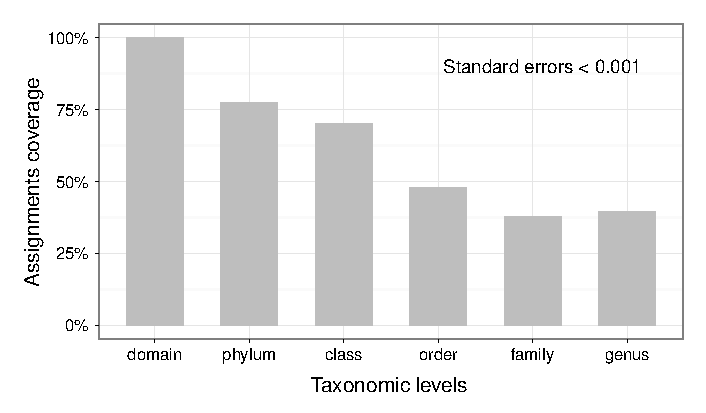
\includegraphics[width=0.7\textwidth]{./figures/Chapter_3/Fig1.eps}
  	\caption{Percentage of reads assigned at each taxonomic level. The number of reads assigned at each taxonomic level has been calculated for each sample. The average number of assigned reads for each taxonomic level from Phylum to Genus is reported. The standard error is shown at the top right of the plot. \label{fig:1rom}}
\end{figure}%
%
\begin{figure}[!tb]
	\centering
	\includegraphics[width=0.8\textwidth]{./figures/Chapter_3/Fig2.eps}
  	\caption{Rarefaction curves. Reported curves have been created by randomly re-sampling the pool of assignments for each sample multiple times and then plotting the average number of genera found in each sample. An increasing step of 1000 assignments has been chosen in order to draw smooth curves. The slopes of each step has been calculated for each sample and reported in the top panel while rarefaction curves have been reported in the bottom one. \label{fig:2rom}}
\end{figure}%

\subsubsection{Differential taxonomic assemblage in core and accessory bacteriome}
To check whether the differences found in the composition of the bacterial community at genus level were also represented at higher taxonomy levels (Table SM3), all genus assignments were collected and collapsed from phylum level to order level. Then, taxonomic differences between core and accessory bacteriomes were inspected (Figure\ref{fig:5rom}). Beginning from phylum level, core and accessory groups displayed significant differences in almost all phyla (only 2 phyla out of 23 did not differentiate between the two groups). In particular, six phyla (\textit{Gemmatimonadetes}, \textit{Elusimicrobia}, OD1, TM7, WS3) were only detected in core bacteriome. Six phyla were present in the accessory bacteriome (\textit{Cyano\-bacteria}, \textit{Aquificae}, \textit{Deino\-coc\-cus\--Ther\-mus}, \textit{Fuso\-bacte\-ria}, \textit{Lenti\-sphaerae}, OP11). The presence of such phyla exclusive of the two pan- acteriome fractions highlight the presence of large taxonomic differences between them, which was also clear from a higher abundance of members of \textit{Plancto\-mycetes}, \textit{Actino\-bacteria}, \textit{Verruco\-micorbia} and \textit{Acido\-bacteria} in the core bacteriome, while the accessory bacteriome comprised more \textit{Firmicu\-tes}, \textit{Clamy\-diae} and \textit{Proteo\-bacteria}. Similar results were obtained by inspecting different taxonomic assemblage at class level. In fact, 16 classes out of 19 showed different occurrences between core and accessory bacteriomes, with 4 (\textit{Erysi\-pelotri\-chia}, \textit{Epsilo\-proteo\-bacteria}, \textit{Holo\-phagae}, Subdivision 5) and 2 (\textit{Acido\-bacteria}, Subdivision 3) classes only present in the accessory and in the core bacteriome, respectively. Finally, almost all detected orders showed a differential occurrence patterns between accessory and core bacteriome, with 7 orders found exclusively in the core dataset and 12 orders found exclusively in the accessory dataset.\\%
\begin{figure}[!tb]
	\centering
	\includegraphics[width=1\textwidth]{./figures/Chapter_3/Fig5.eps}
  	\caption{Phylogenetic dissection of variation of core and accessory bacteriome. Heatmaps report the difference of each taxonomic assignment between the core and the accessory bacteriomes. Differences have been tested using a t-test (with the exclusion of presence/absence patterns). Colors are reflecting the level of the related genus in the heatmap. Green and red colors correspond to high and low abundances values, respectively. The asterisks indicate the p-value threshold in each comparison (one asterisk indicates a p-value lower than 0.05 but higher than 0.001 while two asterisk indicates a p-value lower than 0.001). The open circle indicates a strict presence/absence. \label{fig:5rom}}
\end{figure}%
Finally, to give an insight into the genus-level distribution inside each sample (Table SM4), the number of sequences attributed to each genus was transformed into a relative abundance value. These values were used to display bacterial taxonomic composition in each sample and in each bacteriome (Figure~\ref{fig:6rom}). Results confirmed the overall representation of a conserved core group and of a more scattered accessory genus distribution. Moreover, from this analysis the core group seemed to vary (a little) in relation to the sampling time, while the accessory bacteriome displayed a variation with respect to sampling time to treatment and among repetitions.\\%
\begin{figure}[!tb]
	\centering
	\includegraphics[width=1\textwidth]{./figures/Chapter_3/Fig6.eps}
  	\caption{Relative abundances of genera detected in the core and accessory bacteriomes. Color patterns refer to distinct
901 genera (see Table SM1). In the two panels, abundance values for the core bacteriome and the accessory bacteriome are
reported on the left and the right, respectively. A, B and  C refer to the three treatments. \label{fig:6rom}}
\end{figure}%

\subsubsection{Defining core and accessory bacteriome}
In order to describe the bacterial community structure of the soil under study, the \textit{X} matrix was transformed using the logarithmic function. Thus, a heat map was produced displaying the abundance of all genera in the samples (Figure~\ref{fig:3rom}, Table SM4), which indicated the presence of highly represented and shared taxa (red regions over the whole map) and occasional taxa (regions of the heat map that do not display a uniform color inside the plot). These groups of taxa were defined (as detailed in the Materials and Methods section) as core and accessory bacteriome, respectively. The core (shared) set of genera included those present in all samples (without considering changes in their abundance), while the accessory bacteriome included those genera not present in all samples.\\%
\begin{figure}[!tb]
	\centering
	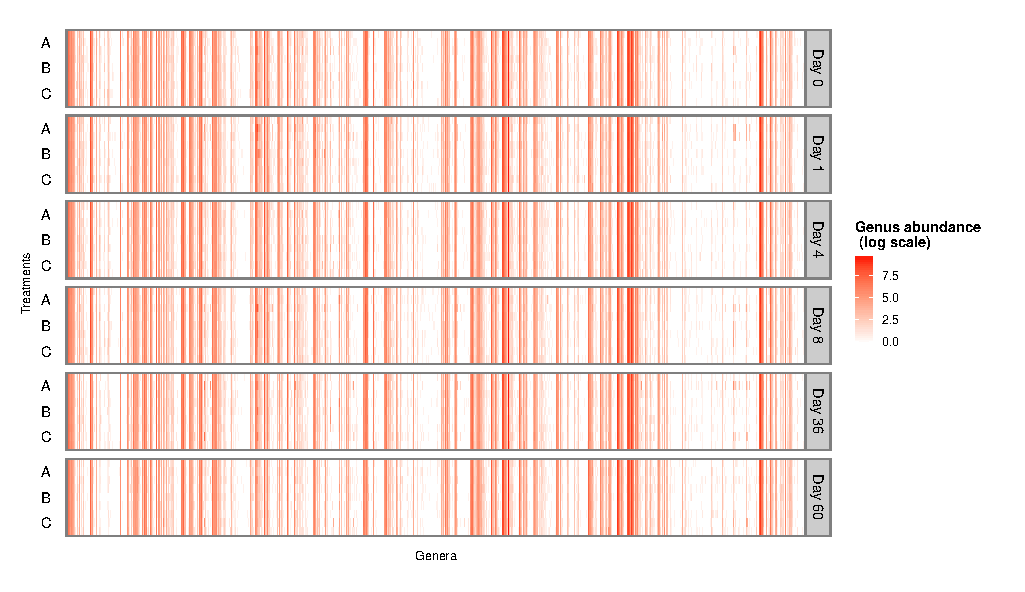
\includegraphics[width=1\textwidth]{./figures/Chapter_3/Fig3.eps}
  	\caption{Bacterial community structure at genus level. The number of assignments at genus level has been transformed using the logarithmic function in order to reduce the range of values. The obtained values have been reported using a heat map representation. As reported in the plot, red color represents high number of assignments (10\textsuperscript{7}), while the white color indicates a low number of assignments (below 10\textsuperscript{1}). Samples have been divided into six blocks following sampling time (grey blocks to the right). Each block has been divided into 9 lines, grouped into three parts following the three simulated environmental conditions (named A, B and C, corresponding to water, Cd 5 mg/kg and 25 mg/kg, respectively). The 901 genera identified in the samples were ordered according to the taxonomic output of RDP Classifier (see Table SM2). \label{fig:3rom}}
\end{figure}%
In terms of number of classified reads, the core and the accessory bacteriome contained 99.4\% and 0.5\% of all sequences classified at genus level, respectively (data not shown). Furthermore, 120 genera were detected in one sample only (less than 0.1\% of the whole sequences); these genera were considered as ``unique'' ones and were excluded from the following analysis (Table SM4). Regarding the core and the accessory bacteriome fractions we have collected 316 core genera (35.1\% of the total)and 465 accessory genera (51.6\% of the total) (Figure~\ref{fig:4rom}).\\%
\begin{figure}[!tb]
	\centering
	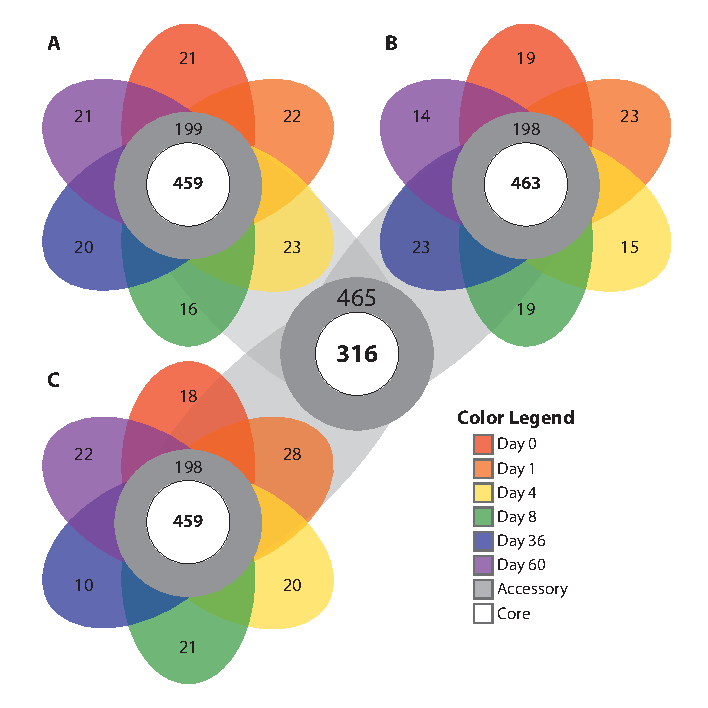
\includegraphics[width=0.7\textwidth]{./figures/Chapter_3/Fig4.eps}
  	\caption{The pan-bacteriome size. Pseudo-Venn diagrams drawn for each treatment dividing each sample according to sampling time. Generated plots report the number of genera found only at a specific time (unique assignments), the number of genera detected at least at two distinct times (accessory assignments) and the number of genera detected in all samples regardless sampling time (core assignments). The two groups reported in the middle of the three Venn diagrams are the accessory and the core groups defined with respect to the whole bacterial community, regardless sampling time and treatment. The three Venn diagrams marked with the letters ``A'', ``B'' and ``C'' are referring to the 3 treatment conditions (0, 5, 25 mg/kg of Cd). \label{fig:4rom}}
\end{figure}%

\subsubsection{Effect of sampling time and treatment on the whole pan-bacteriome components}
We then considered the differential response of core and accessory bacteriome when comparing the three different mesocosms (treatment A, B, and C, with [Cd\textsuperscript{2+}] at 0, 5 and 25 mg kg\textsuperscript{-1}, respectively). Two analyses were performed by CCA: one considering all samples collected for the analysis (replicates included) and one pooling the 3 replicates of each condition into a single observation. Both factors (sampling time and treatment) were fitted onto the two ordination analyses described above (Figure~\ref{fig:7rom}). Results showed a tendency of the non-pooled samples to preferably cluster based on sampling time rather than on treatments. On the other hand, the pooled samples displayed an opposite behavior; in fact, they tended to cluster following the treatments (A, B, C) but not the sampling time. These contrasting results could be due to the high level of heterogeneity in the accessory bacteriome assignments. As shown in the bacterial communities analysis performed above (Figure~\ref{fig:6rom}), the accessory group displays a very scattered bacterial distribution even inside the same temporal and treatment conditions. If this effect is minimized by pooling the 3 replicates inside a single sample even the effect of randomness is minimized. On the contrary, if this effect is not reduced, replicates of the same conditions result in a high degree of overlap in the ordination analysis.\\%
\begin{figure}[!tb]
	\centering
	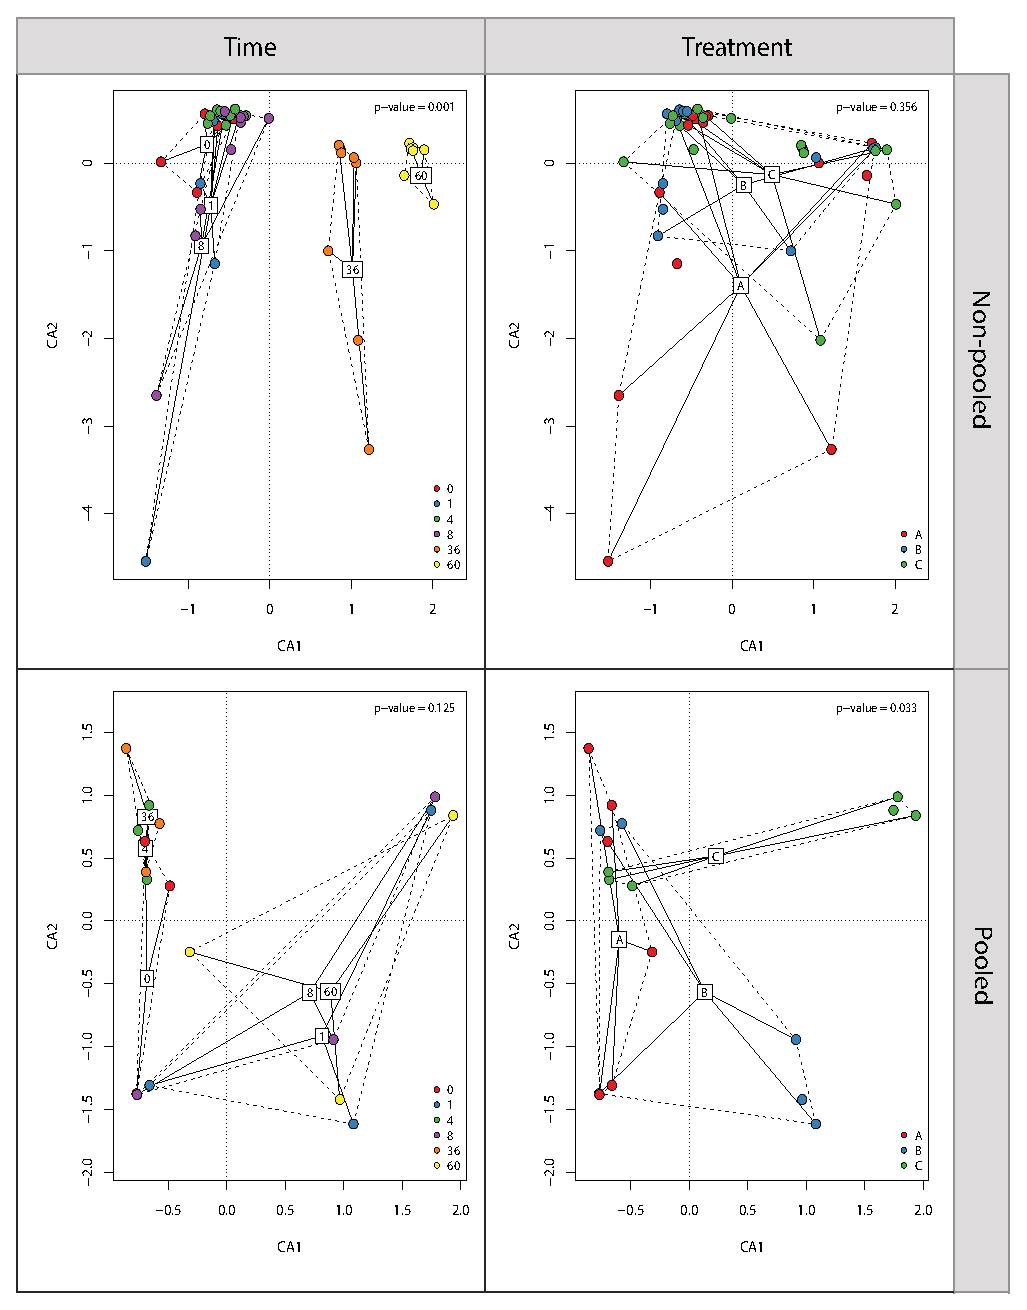
\includegraphics[width=0.9\textwidth]{./figures/Chapter_3/Fig7.eps}
  	\caption{Effect of environmental variables on the pan-bacteriome assemblage. Canonical Correlation Analysis of the whole bacterial community are reported. The four plots are divided according to the time and treatment factor (vertical division) and according to the dataset used (horizontal division). In particular, the two plots in the bottom panel report the ordination analysis based on the pooled dataset (samples with the same conditions were pooled together) whereas the two plots in the top panel report the ordination analysis based on the whole bacterial community (all samples). P values derived from an environmental fitting analysis onto the bacterial dataset where reported in the top right corner of each plot. \label{fig:7rom}}
\end{figure}%

\subsection{Discussion}
It is now widely accepted that bacterial communities are composed by an assembly of resident taxa, those being slightly affected by environmental variables, and by occasional/fluctuating taxa, those varying among samples \cite{logares2012biogeography}. Often resident taxa are the most abundant, while occasional taxa tend to be rare \cite{gobet2011diversity}. Recently, habitat specialization has been used to classify and provide insight into the ecological behavior of microbial taxa \cite{szekely2014importance}.\\
To better describe the assemblage of bacterial communities as a sum of resident and occasional taxa, we have used a conceptual framework analogous to the pangenome concept \cite{tettelin2008comparative}, which is used for describing bacterial genomes belonging to the same species as sum of a common gene set (core genome) and of a dispensable/accessory gene set. In particular, we evaluated the presence of core and accessory bacteriomes in a set of three soil mesocosms followed over time.\\
The presence of two main fractions of the bacterial community was highlighted; one (the core), including the resident taxa while the other (accessory) composed of occasional taxa. The accessory taxa were by far fewer than the core taxa, considering the number of sequence assigned to each group. Since our experimental dataset included three different mesocosms (treatment A, B, and C, with [Cd\textsuperscript{2+}] at 0, 5 and 25 mg kg\textsuperscript{-1}, respectively) followed for a relatively short time (60 days), occasional taxa could then include some fast growing/responding strains with rapid cycles of extinction (below amplification threshold)/colonization (above amplification threshold), as postulated for r-strategy taxa \cite{safriel1980criteria}, while the core bacteriome could include taxa with a k-strategy of growth. Treatment with high concentrations of Cd (A, B, C) did not substantially alter the diversity (Table SM2) or the taxonomic assemblage of bacterial communities (Figure~\ref{fig:7rom}). However, temporal shifts were detected which allowed to identify taxonomic signatures for the core and the accessory bacteriome. The core bacteriome was richer in members of phyla \textit{Planctomycetes}, \textit{Actinobacteria}, \textit{Verrucomicorbia} and \textit{Acidobacteria}, than the accessory bacteriome. The accessory bacteriome included more members of \textit{Firmicutes}, \textit{Clamydiae} and \textit{Proteobacteria } (here in particular the order \textit{Pseudomonadales}) than the core bacteriome. Moreover, the differential occurring taxa included 16S rRNA gene sequences from uncultured divisions, for which few or no functional information are available. In particular, \textit{Armatimonadetes} (previously known as candidate phylum OP10) \cite{tamaki2010armatimonas}, OD1, TM7 and WS3 were only present in the core microbiome, suggesting they were scarcely or not affected by time in the hree environmental condition tested (mesocosms of A, B and C types). These phyla may include strains potentially being ``seeds'' for maintaining soil bacterial functionality and with low replication times, as k- trategists, similarly to the habitat generalist taxa, recently discussed for rock pools \cite{szekely2014importance}.\\
Concerning the accessory bacteriome, several taxonomic orders were more represented, with respect to the core bacteriome, or exclusively found in the accessory bacteriome (Figure~\ref{fig:5rom}). For instance, genera of the classes \textit{Betaproteobacteria} (as \textit{Burkholderiales} and \textit{Methylophylales}), and \textit{Bacilli} (\textit{Bacillales}) and \textit{Clostridia} were more abundant in the accessory bacteriome. These taxa may include strains that are r-strategist of selection and/or strains more sensitive to environmental perturbation. Therefore, their number may vary consistently between samples, dropping below the PCR amplification threshold in some particular conditions. Moreover, since many of these taxa (as \textit{Bacilli} and \textit{Clostridia}) may produce spores, which have a lower DNA extraction yield than cells \cite{dineen2010evaluation}, we cannot exclude that some of the fluctuations observed in the accessory bacteriome for \textit{Bacilli} and \textit{Clostridia} may indeed be due to the differential presence of spores and living cells along sampling times. Additionally, a possible higher level of stochasticity of accessory bacteriome fluctuation can be inferred when comparing A, B and C treatments. In fact, the different results obtained in the comparison of treatments in pooled and non-pooled samples (Figure~\ref{fig:7rom}) could indeed be ascribed to the higher variability of replicas for the accessory fractions (see also Figure~\ref{fig:6rom}). However, from the presented data it is not possible to draw so far general conclusions about the taxa which may be part of the core and of the accessory bacteriome in soil, because nutrient and other environmental conditions may differentially affect the bacterial taxa. Other studies, employing soil mesocosms with different nutrient availability (as for instance organic carbon and nitrogen) and different type of  stressors (i.e. salinity, temperature, other heavy-metals, etc.) should be performed in order to better evaluate the extent of core vs. accessory bacteriome and their respective taxonomic compositions.\\
Moreover, the metabarcoding method here described only included phylum- to genus-level comparisons. Therefore, it is possible that some species or strains, belonging to identified genera, may have different responses to the treatments that were not observed by the analyses here described.\\
Future studies focused on single genera, could then be useful in providing insights into the biological interpretation of the core/accessory bacteriome model in a narrow taxonomic range.\\
In conclusion, the concept of the pan-bacteriome as the sum of all taxa from the same soil at different times is proposed. This approach can allow identifying a core (stable) and an accessory (variable) pool of taxa, with a response to time and to different environmental conditions (mesocosms of A, B and C types). Core and accessory bacteriomes represented roughly 1/3 and 1/2 of the taxa detected in our dataset, respectively. These two bacterial fractions show a divergent number of assigned sequences; in particular the core group contains the 99.4\% of the sequences assigned at genus level while the accessory group contained only the 0.5\%. These data suggest a large flexibility of the pan-bacteriome in our experimental conditions. Furthermore, the two groups of soil bacteriome show a different taxonomic assemblage, which may reflect a different ability of these pools to persist in soil. We propose that , the pan-bacteriome model of the bacterial community dynamics could be a useful approach for highlighting potential ecological (and functional) differences among bacterial taxa thriving in soil.\\

\subsubsection{Acknowledgments}
This work was supported by a grant from the Ente Cassa di Risparmio di Firenze (Grant n{\textdegree} 2010/4384 ``Centro di Metagenomica del suolo''). 


%%-----------
%% Backmatter
%%-----------
\backmatter
\chaptermark{Bibliography}
\renewcommand{\sectionmark}[1]{\markright{#1}}
\bibliographystyle{unsrt}                           %Use alpha codes for references
\sectionmark{Bibliography}
\addcontentsline{toc}{chapter}{Bibliography}        %Force addition of Bibliography to TOC    
\bibliography{References}